\thispagestyle{empty}
\newlength{\headsepold}
\setlength{\headsepold}{\headsep}
\setlength{\headsep}{-1.26cm}
\newgeometry{left=1.28cm,right=1.28cm,top=1.28cm,bottom=0cm}
\definecolor{tum_blau_2016}{RGB}{0,101,189}
\begin{center}
{\sffamily
\fontsize{18}{18}\selectfont 
\begin{minipage}[b]{120mm}
\ifthenelse{\boolean{bmgerman}}{
\small \textcolor{tum_blau_2016}{Lehrstuhl f{\"u}r Baumechanik \\
TUM School of Engineering and Design \\
Technische Universit{\"a}t M{\"u}nchen}}
{
\small \textcolor{tum_blau_2016}{Chair of Structural Mechanics \\
TUM School of Engineering and Design \\
Technical University of Munich}
}
\end{minipage}
% BM Logo
%
\includegraphics[width=1.2cm, keepaspectratio=true]{bvlogo} 
\includegraphics[width=1.5cm, keepaspectratio=true]{bmlogo} \hfill 
	%\begin{minipage}[b]{80mm}
 %\small \centering Lehrstuhl f{\"u}r Baumechanik - TU M{\"u}nchen \\ 
  %\end{minipage}
% TUM Logo
 \hfill \includegraphics*[height=1.28cm, keepaspectratio=true]{TUM_Logo_blau_rgb_2016}
\vspace{0.5cm}
%\hrule
%Text mittig ausgerichtet
%\begin{center}
%\vspace{4cm}
%{\huge \textbf{ \veranstaltung }}\\[4 pt]
%\Large \lehrer \\%\sc
%\vspace{0.5cm}
%\Large{\semester}\\
%\end{center}}
%\end{center}

%Text linksbündig
}
\end{center}
\vspace{3cm}
{\sffamily
\begin{doublespace} %Größerer Zeilenabstand, falls Veranstaltungstitel umgebrochen werden muss
{\huge{\textbf{\veranstaltung}}}%
\end{doublespace}
\Large \lehrer 
\ifdef{\assistent}{\\[.1cm] \normalsize \assistent}{}
\\[.9cm]
\large \semester %\normalize
}

% Uhrenturm Bild
\enlargethispage{3.5cm}
\vspace{2cm}
\begin{figure}[h]
\begin{addmargin}{-2cm}
\flushright
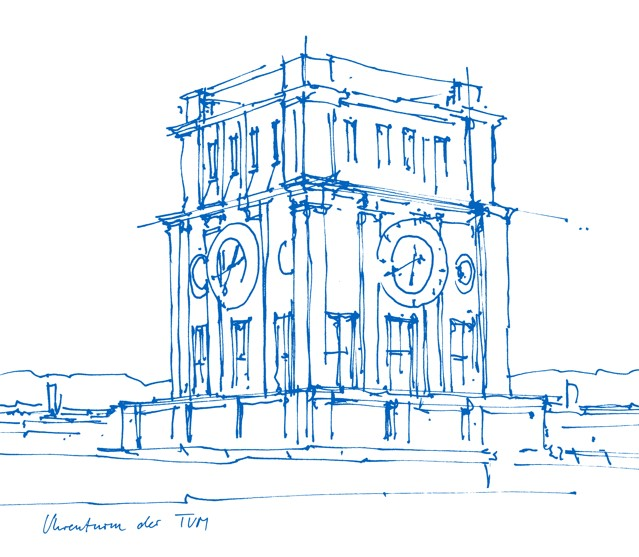
\includegraphics[width=14cm, keepaspectratio=true]{Bild_TUM_Uhrenturm_2016}%width 19cm
\end{addmargin}
\end{figure}
\vfill
%\begin{flushleft}
%\href{http://www.sqk.bv.tum.de}{
\includegraphics[height=3.1cm, keepaspectratio=true]{deinvorteil}}
%\end{flushleft}
\restoregeometry
\newpage
\setlength{\headsep}{\headsepold}
